%% LaTeX2e class for student theses
%% sections/conclusion.tex
%% 
%% Karlsruhe Institute of Technology
%% Institute for Program Structures and Data Organization
%% Chair for Software Design and Quality (SDQ)
%%
%% Dr.-Ing. Erik Burger
%% burger@kit.edu
%%
%% Version 1.3.3, 2018-04-17

\chapter{Conclusion}
\label{ch:Conclusion}
Correlation analysis is one of the fundamental task of Data Mining. It aims at discovering and summarizing the relationship between the attributes of a data set. Knowing the relationship between a set of variables, one can infer useful knowledge about external, a priori unknown outcomes. The evolving nature of streams and the high-dimensionality are two main challenges of analyzing high-dimensional data streams.\\
The goal of this thesis is the development of an interface for visualization of correlation in high-dimensional streams. We compare three different visualization methods through this interface: Heatmap, Bar Graph and Force-Directed-Graph. Our interactive interface reflects a tendency of the data correlation by visualization throughout the time. Users are able to choose a certain period of time to perform the correlation analysis and visualization. It is easy and quick for users to find pairs of attributes with strong correlations and also to see the evolution of data set during the time. This interface makes it possible to have a first glance at the data and provides some basic information before starting detailed analysis.\\
With the help of feedback from controlled user study, more useful functions can be added to our interface in order to ease the correlation analysis. Also, this interface can have more visualization methods than Heatmap, Bar Graph and Force-Directed-Graph and the current existing visualization methods can still be improved. In our thesis, we only focus on pairwise relationships and the correlations between more than two variables may remain to be discovered in the future work.\\



%% -------------------
%% | Example content |
%% -------------------

%This is the SDQ thesis template.
%For more information on the formatting of theses at SDQ, please refer to
%\url{https://sdqweb.ipd.kit.edu/wiki/Ausarbeitungshinweise} or to your advisor.

%\section{Example: Citation}
%\label{sec:Introduction:Citation}
%A citation: \cite{becker2008a} For referencing, see \autoref{sec:Introduction:Figures}

%\section{Example: Figures}
%\label{sec:Introduction:Figures}
%\begin{figure}[h]
%	\centering
%	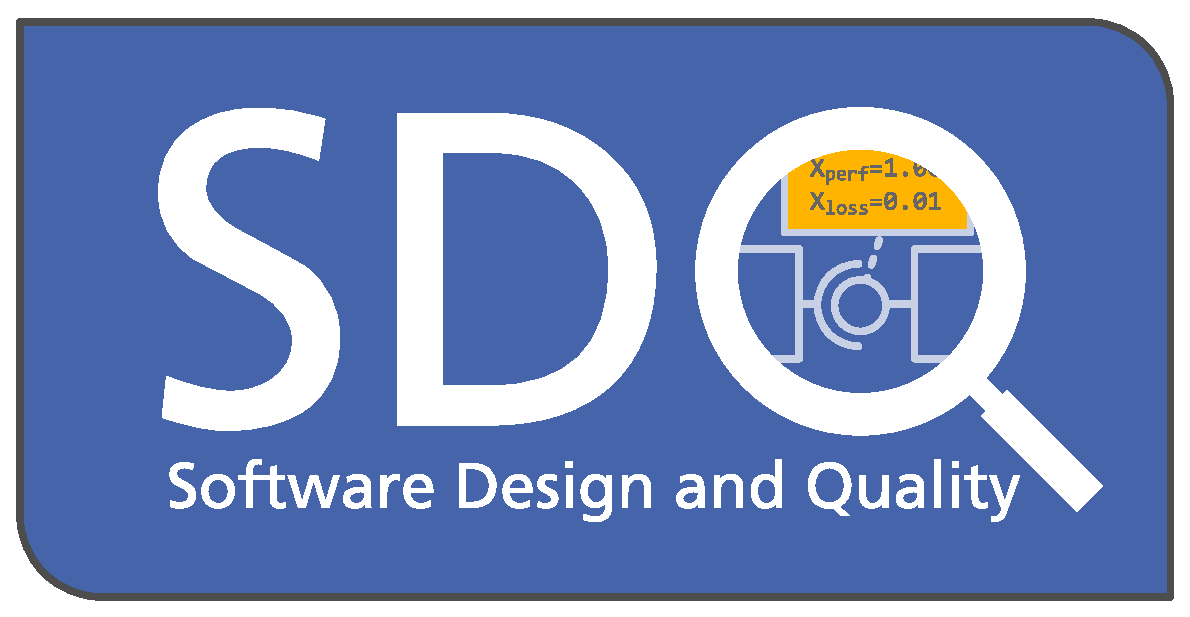
\includegraphics[width=4cm]{logos/sdqlogo}
%	\caption{SDQ logo}
%	\label{fig:sdqlogo}
%\end{figure}

%A reference: The SDQ logo is displayed in \autoref{fig:sdqlogo}. (Use \code{\textbackslash autoref\{\}} for easy referencing.) 

%\section{Example: Tables}
%\label{sec:Introduction:Tables}
%\begin{table}[h]
%	\centering
%	\begin{tabular}{r l}
	%	\toprule
	%	abc & def\\
	%	ghi & jkl\\
	%	\midrule
	%	123 & 456\\
	%	789 & 0AB\\
	%	\bottomrule
%	\end{tabular}
%	\caption{A table}
%	\label{tab:atable}
%\end{table}

%\section{Example: Todo-Note}
%Meaningless text.

%\section{Example: Formula}
%One of the nice things about the Linux Libertine font is that it comes with a math mode package.
%\begin{displaymath}
%f(x)=\Omega(g(x))\ (x\rightarrow\infty)\;\Leftrightarrow\;
%\limsup_{x \to \infty} \left|\frac{f(x)}{g(x)}\right|> 0
%\end{displaymath}

%% --------------------
%% | /Example content |
%% --------------------

%% -------------------
%% | Example content |
%% -------------------
%The content chapters of your thesis should of course be renamed. How many chapters you need to write depends on your thesis and cannot be said in general.

%Check out the examples theses in the SDQWiki:

%\url{https://sdqweb.ipd.kit.edu/wiki/Abschlussarbeit/Studienarbeit}

%Of course, you can split this .tex file into several files if you prefer. 








